\chapter{分散式系統}
\renewcommand{\baselinestretch}{10} %設定行距
%\section{前言}
\par
\renewcommand{\baselinestretch}{1} %設定行距
\twelve 要合作就必須溝通與協調,俗話說合作就是力量大,但是溝通與協調不僅僅是一種本能,更是一種能力。這就是分散式運算的問題來源,在分散式環境中,合作對象是分散各地的電腦,在這些電腦透過網路連接在一起,每台電腦都能讀立運行,且同時也能藉由分散式系統來進行合作,若以一個基層人員而言,需要將上級、同級、下級,甚至客戶,的每一件事項在對應的部分做串聯,甚至獨立解決,而產生一加一大於二的成效。
\par

\renewcommand{\baselinestretch}{20} %設定行距
\section{分散式系統的基本架構}
\par
\renewcommand{\baselinestretch}{1} %設定行距
\twelve 分散式系統則是將硬體設備或軟體元件,分布在不同的網路主機上,藉著彼此之間的網路進行通訊與協調的系統。可以想像成一群獨立的電腦系統集中起來對外提供服務,但對於使用者而言,就像是在使用一台強大的主機,就是透過網路將許多台電腦資源連結起來。當有一個大型任務需要執行時,會先將任務分割成許多小型運算工作,再分派給所有的電腦執,最後再將所有執行的結果彙整。網格運算與雲端運算即是分散式系統常見的應用。而通常更複雜的分散式系統也是由以下三個系統架構(圖.\ref{fig.基本架構})組何而成。
\\
\begin{itemize}
	\item 中心化網路(CENTRALIZED)
	\item 去中心化網路(DECENTRALIZED)
	\item 分散式系網路(DISTRIBUTED)
\end{itemize}
\par

\clearpage%換頁
\renewcommand{\baselinestretch}{2} %設定行距
\begin{figure}[hbt!]
\begin{center}
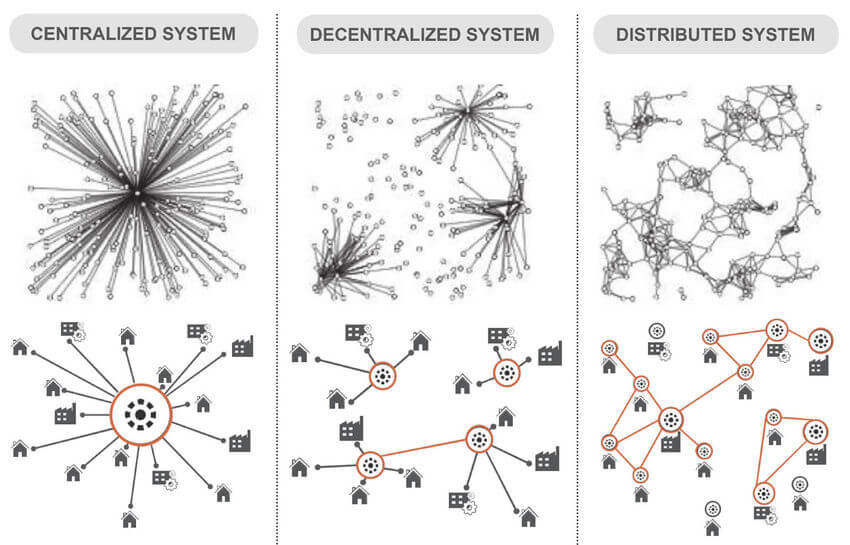
\includegraphics[width=6in]{1}
\caption{\large 基本架構}\label{fig.基本架構}
\end{center}
\end{figure}
\par

\renewcommand{\baselinestretch}{20} %設定行距
\section{版本控制}
\par
\renewcommand{\baselinestretch}{1} %設定行距
\twelve 版本控制是一種紀錄資料變化或內容改變的完整歷程,並且每次改動將賦予一個新代碼,當版本控制系統開始使用時,是所有開發者合作的一種方式,共用一個儲存庫(Repository)的概念,儲存庫可以視為一種資料庫,開發者通常會利用版本控制來追蹤、維護原始碼、檔案以及設定檔等等的改動。而通常版本控制分為(圖\ref{fig.版本控制})以下兩種形式。
\\
\par
\renewcommand{\baselinestretch}{1.7} %設定行距
\begin{figure}[hbt!]
\begin{center}
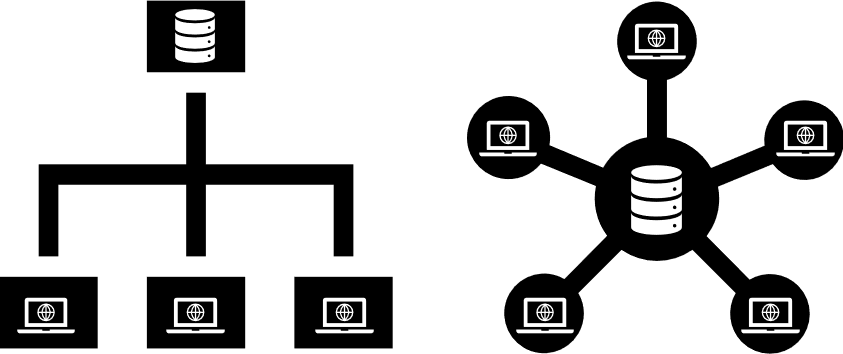
\includegraphics[width=3in]{2}
\caption{\large 集中式版本控制(左)\enspace vs.分散式版本控制(右)}\label{fig.版本控制}
\end{center}
\end{figure}
\par
\renewcommand{\baselinestretch}{1} %設定行距
\twelve 而集中式版本控制與分散式版本控制系統的功能都包含了,同步、追溯、以及備份,相差不大,最主要的差別在於集中式的資料庫是集中控管,因此需要透過網路連結主機,開發者需要提交檔案或要對資料庫做一些其他的操作,都必須要在能夠連接上網路的環境下進行做操作,因此在網路環境或速度不佳的地區,會影像到開發效率。而分散式的資料庫允許不只一份,事實上,每個開發者都可以在自己的主機上建立儲存庫,因此版本代碼會記錄在儲存庫上,因此可以在無需網路環境下進行操作,需要進行遠端同步時,才需要網路連線,而開發者才能進行推送(push)的操作到其他儲存庫上,而其他開發者需要在網路連線下,才能進行拉取(pull)的操作,在各自進行開發的工作。
\par

\renewcommand{\baselinestretch}{20} %設定行距
\section{事件的排序問題}
\par
\renewcommand{\baselinestretch}{1} %設定行距
\twelve 分散式系統在事件的排序上是一個很重要的部分。在單一主機系統下,我們可以由系統時鐘來判斷兩個事件發生的前後順序,例如處理元需要使用某個資源之前,需要擁有使用權,所以使用資源的事件一定得發生在擁有資源使用權的事件後。在分散式系統中沒有時鐘,所以在理論上必須對基本的觀念與邏輯有一定的能力,才不製造資料的衝突。
\\
\par
\renewcommand{\baselinestretch}{1} %設定行距
\twelve 當本地儲存庫推送遠端時,因為遠端儲存庫資料以經被其他協同者更新,所以本地儲存庫推送時,會造成衝突,而無法成功推送如(圖\ref{fig.衝突})。
\\
\par
\renewcommand{\baselinestretch}{1.7} %設定行距
\begin{figure}[hbt!]
\begin{center}
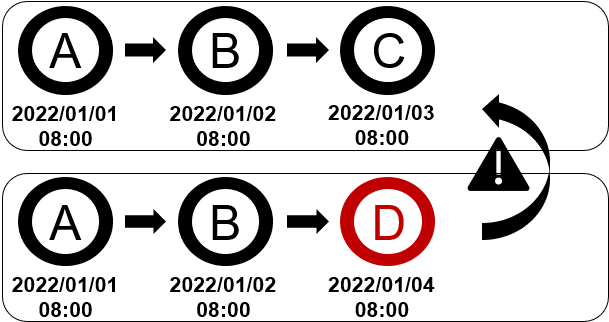
\includegraphics[width=4in]{3}
\caption{\large 遠端儲存庫(上)、本地端儲存庫(下)}\label{fig.衝突}
\end{center}
\end{figure}
\par
\renewcommand{\baselinestretch}{1} %設定行距
\twelve 這時候,需要遠端儲存庫進行合併,若直接覆蓋,則會造成C直接消失,然後在進行推送的操作,而遠端就進行同步的動作如(圖\ref{fig.衝突})。
\\
\par
\renewcommand{\baselinestretch}{1.7} %設定行距
\begin{figure}[hbt!]
\begin{center}
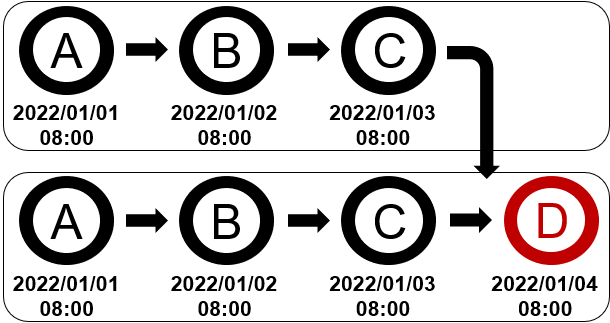
\includegraphics[width=4in]{4}
\caption{\large 遠端儲存庫(上)、本地端儲存庫(下)}\label{fig.解決衝突}
\end{center}
\end{figure}
\par
\renewcommand{\baselinestretch}{1} %設定行距
\twelve 執行合併會自動合併修改或更新資料,但也有不能自動合併的時候。若遠端儲存庫和本地儲存庫的同一個地方都發生修改的情況下,這時,因為不能自動判斷要導入哪一個修改內容,於是就發生錯誤。而發生衝突的部分,需要以手動或其他方式修改內容,在執行合併的操作,就可以推送資料,而遠端就能進行同步動作。
\par